\documentclass[12pt,a4paper]{article}
\usepackage[UTF8]{ctex}
\usepackage{amsmath,amssymb}
\usepackage{xcolor}
\usepackage{hyperref}
\usepackage{geometry}
\usepackage{graphicx}
\geometry{margin=2.5cm}

\title{Quantum Scheduling / 量子调度}
\author{QuoNic}
\date{}

\begin{document}
\maketitle

\begin{center}
\textbf{Compilation / 编译} | 难度：中级 | 预计时间：10 分钟
\end{center}

\tableofcontents
\newpage

\section{为什么需要？}

量子调度用于优化量子门的执行顺序。

\subsection{经典局限}
\begin{itemize}
  \item 量子门的执行顺序会影响电路深度
  \item 需要优化调度
\end{itemize}

\subsection{量子优势}
\begin{itemize}
  \item 量子调度可以减少电路深度
  \item 提高执行效率
  \item 减少噪声影响
\end{itemize}

\subsection{实际应用}
\begin{itemize}
  \item 量子编译
  \item 电路优化
  \item 硬件执行
\end{itemize}

\section{快速上手}

\begin{verbatim}
from quonic.compile import schedule

# 量子调度
result = schedule(circuit)
print(f'Scheduled circuit: {result.circuit}')
print(f'Depth: {result.depth}')
\end{verbatim}

\textbf{预期输出}：
\begin{verbatim}
Scheduled circuit: ...
Depth: 3
\end{verbatim}

\section{原理详解}

\subsection{电路图}

\begin{center}
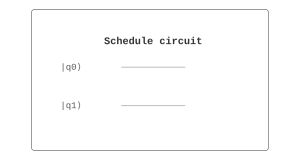
\includegraphics[width=0.6\textwidth]{../../images/schedule_circuit.svg}
\end{center}

\subsection{数学推导}

量子调度：
\begin{equation}
\text{depth} = \max_i \text{layer}(i)
\end{equation}

其中 $\text{layer}(i)$ 是第 $i$ 个门的层。

\subsection{几何解释}

量子调度在时间轴上安排量子门的执行顺序。目标是最小化电路深度。

\section{代码详解}

\begin{verbatim}
from quonic.compile import schedule

# schedule(circuit, method)
# circuit: 量子电路
# method: 调度方法 ('asap', 'alap', 'critical_path')

result = schedule(
    circuit=circuit,
    method='asap'
)

# result.circuit: 调度后的电路
# result.depth: 电路深度
# result.schedule: 调度表
print(f'Scheduled circuit: {result.circuit}')
print(f'Depth: {result.depth}')
\end{verbatim}

\section{进阶用法}

\subsection{场景 1：不同调度方法}

\begin{verbatim}
from quonic.compile import schedule

# 不同调度方法
r1 = schedule(circuit, method='asap')
r2 = schedule(circuit, method='alap')
r3 = schedule(circuit, method='critical_path')
\end{verbatim}

\section{适用场景}

\subsection{量子编译}

量子调度用于量子编译器，优化量子门的执行顺序。

\subsection{电路优化}

量子调度可以减少电路深度，提高执行效率。

\section{常见问题}

\subsection{量子调度和经典调度有什么区别？}

量子调度需要考虑量子门的依赖关系和量子比特的约束。

\subsection{量子调度的性能如何？}

量子调度的性能取决于调度方法和电路特性。

\section{学习路径}

\subsection{前置知识}
\begin{itemize}
  \item 量子电路
  \item 量子门
  \item 量子编译
\end{itemize}

\subsection{继续学习}
\begin{itemize}
  \item 量子编译
  \item 电路优化
  \item 量子硬件
\end{itemize}

\section{完整示例代码}

\subsection{示例 1：基本量子调度}

\begin{verbatim}
from quonic.compile import schedule

result = schedule(circuit)
print(f'Scheduled circuit: {result.circuit}')
\end{verbatim}

\section{下载}

\begin{itemize}
  \item [schedule.py](https://github.com/ChrisLee0721/QuoNic/blob/main/examples/schedule/schedule.py)
\end{itemize}

\end{document}
